\documentclass[journal]{IEEEtran}
\usepackage{lipsum} % 示例中使用的假文宏包
\ifCLASSINFOpdf
\else
   \usepackage[dvips]{graphicx}
\fi
\usepackage{url}

\hyphenation{op-tical net-works semi-conduc-tor}
\usepackage{pdfpages} % 添加pdfpages宏包
\usepackage{graphicx}
\usepackage{caption}
\usepackage{mathtools}
\usepackage{xcolor}
\usepackage{amsmath}
\usepackage{listings}
\usepackage{matlab-prettifier}
\usepackage{float}
\usepackage{subfigure}



\lstdefinestyle{vhdlStyle}{
    language=VHDL,
    basicstyle=\small\ttfamily,
    keywordstyle=\color{blue},
    commentstyle=\color{green!70!black},
    stringstyle=\color{purple},
    emph={ENTITY, IS, PORT, IN, OUT, END, ARCHITECTURE, OF, BEGIN, PROCESS, SIGNAL, IF, THEN, ELSE, ELSIF, WHEN, OTHERS},
    emphstyle={\color{magenta}},
    showspaces=false,
    showstringspaces=false,
    frame=none,
    backgroundcolor=\color{lightgray!25},
    breaklines=true,
    breakatwhitespace=false,
    tabsize=4
}  
\lstset{style=vhdlStyle}
\begin{document}

\title{\color[rgb]{0,0.6,1}Digital System Design Course Labora (March 2024)}

\author{12110405   Zhewei Chen}
%\thanks{This paragraph of the first footnote will contain the date on which you submitted your paper for review. It will also contain support information, including sponsor and financial support acknowledgment. For example, ``This work was supported in part by the U.S. Department of Commerce under Grant BS123456.'' }
%\thanks{The next few paragraphs should contain the authors' current affiliations, including current address and e-mail. For example, F. A. Author is with the National Institute of Standards and Technology, Boulder, CO 80305 USA (e-mail: author@boulder.nist.gov).}
%\thanks{S. B. Author, Jr., was with Rice University, Houston, TX 77005 USA. He is now with the Department of Physics, Colorado State University, Fort Collins, CO 80523 USA (e-mail: author@lamar.colostate.edu).}}

\markboth{EE332 Digital System Design}
{Shell \MakeLowercase{\textit{et al.}}: Bare Demo of IEEEtran.cls for IEEE Journals}
\maketitle

\begin{abstract}
This lab report will continue the discussion of the discrete fourier transform DFT and introduce fast fourier transform(FFT). 
\end{abstract}

\begin{IEEEkeywords}
   Full-adder, Vivado, VHDL, Simulation
\end{IEEEkeywords}


\IEEEpeerreviewmaketitle



\section{Introduction}
\IEEEPARstart{T}{his} laboratory will continue the discussion of the DFT and will introduce the Fast Fourier Transform (FFT). Firstly, we try to shift the frequency range and horizontal axis to make our DFT values plot more similar to the conventional DTFT plot. Then, we researched how the zero padding affects our DFT values plot. When studying FFT, we first explored the divide and conquer method to accelerate DFT. Then, by employing a recursive approach, we implemented the aforementioned method to achieve an FFT of lengths 2, 4, 8.
Additionally, we will study how to use zero padding to compute the FFT of lengths $N$, where $N=1,2,3\dots$.




\section{Experimental Contents}
\label{sec:guidelines}


\subsection{Continuation of DFT Analysis}
This section continues the analysis of the DFT started in the previous week's laboratory.

DFT: \(\displaystyle ~~~~~~\) \(X_N[k] = \sum\limits_{n=0}^{N-1} x[n]e^{-j2\pi kn/N}\)

\subsubsection{Shifting the Frequency Range } 
$~$


First, create a Hamming window \(x\) of length \(N = 20\), then use the Matlab function DFTsum to compute the 20-point DFT of \(x\). 
Plot the magnitude of the DFT, \(\lvert X_{20}[k]\rvert\), versus the index \(k\).
\begin{figure}[H]
   \centering
   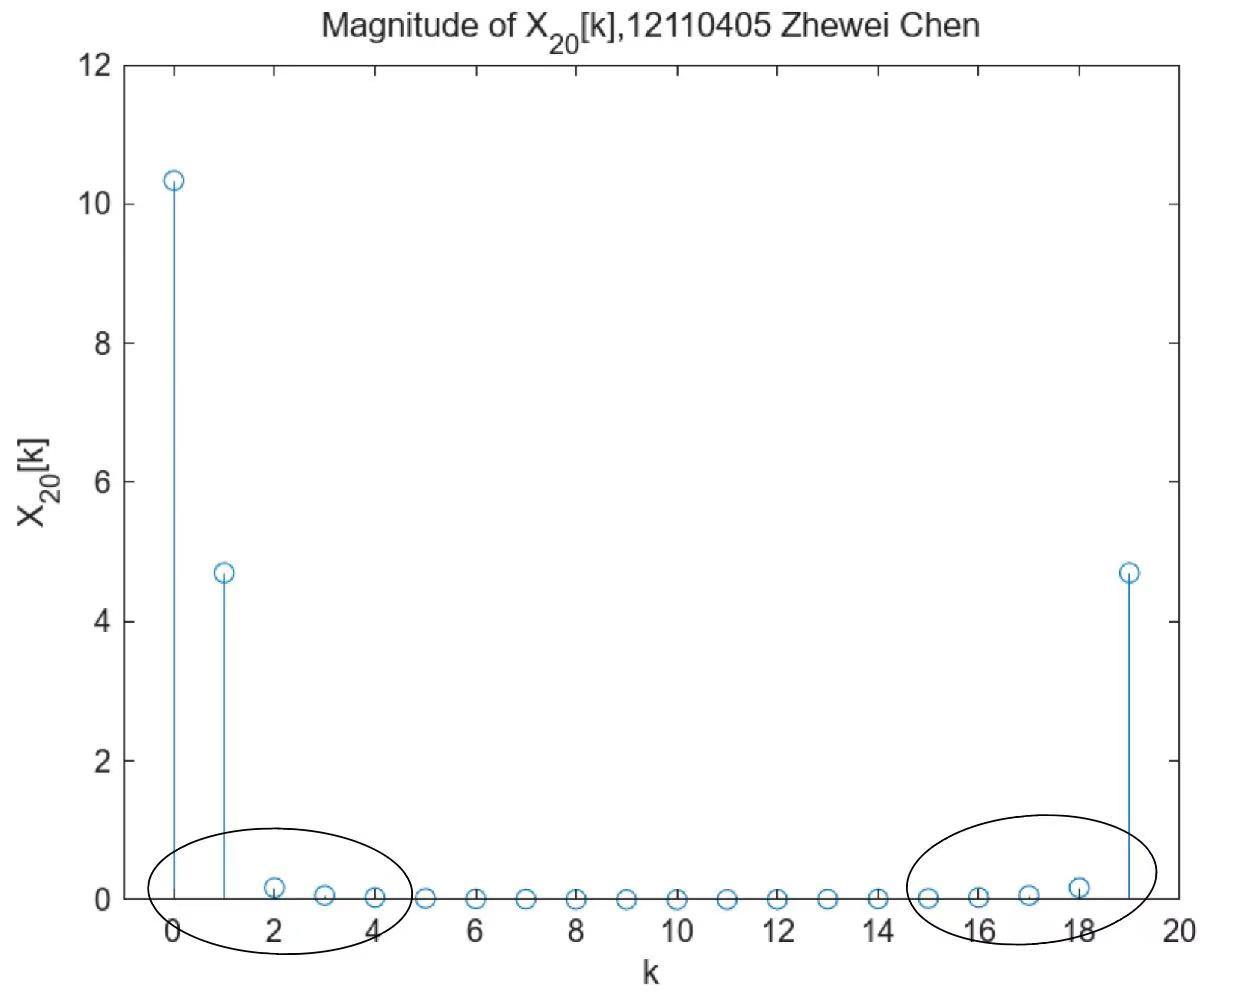
\includegraphics[width=0.4\textwidth]{521.png} % 将"your_image.png"替换为您的PNG图片文件名
\caption{Plot of \(\lvert X_{20}[k]\rvert\) versus the index \(k\)}
   \label{fig:1}
 \end{figure}

\textcolor[rgb]{0,0.6,1}{Analysis:}

\textcolor[rgb]{0,0.6,1}{1 -} The regions of low frequency component is shown in the circles of Fig. 1.

\textcolor[rgb]{0,0.6,1}{2 -} There exists two disadvantages of our DFT values plots.

\textcolor[rgb]{0,0.6,1}{2.1} The frequency range of the DFT is from 0 to \(2\pi\), which is different from the conventional DTFT plot, which is from \(-\pi\) to\(\pi\). 

\textcolor[rgb]{0,0.6,1}{2.2} The horizontal axis of the DFT values plot is against to k rather than \(\omega\).

Then we can write a MATLAB fourier called $\mathbf{DTFTsamples.m}$ to get the plot of DTFT samples using $\mathbf{DFTsum.m}$ and $\mathbf{fftshift()}$ to resolve the two problems above.

\begin{lstlisting}[title={DTFTsamples.m},style=Matlab-editor]
   function [X,w] = DTFTsamples(x)
   N = length(x);
   k = 0:N-1;
   w = 2*pi*k/N;
   w(w>=pi)=w(w>=pi)-2*pi;% shift the range from [0,2*pi] to [-pi,pi]
   w = fftshift(w);
   X = fftshift(DFTsum(x));
   display(w);display(X);
   end 
\end{lstlisting}

\begin{figure}[H]
   \centering  
   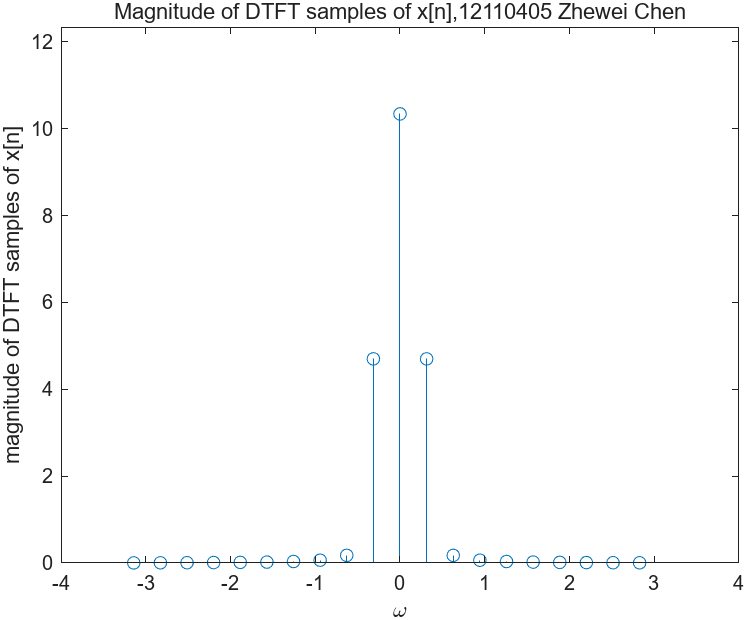
\includegraphics[width=0.4\textwidth]{522.png} % 将"your_image.png"替换为您的PNG图片文件名
\caption{  Plot of DTFTsamples of hamming window with N = 20}
   \label{fig:2}
 \end{figure}

\textcolor[rgb]{0,0.6,1}{Analysis:}

\textcolor[rgb]{0,0.6,1}{1 -} By transforming $k$ to $\omega$ by $\omega =2\pi k/N$,the plot is against $\omega$ now.

\textcolor[rgb]{0,0.6,1}{2 -} Using function $\mathbf{fftshift()}$ to shift both $\omega$ and DTFTsamples, we can get the plot in the range of $[-\pi,\pi]$.


\subsubsection{Zero Padding}
 $~$

This section we will use finite duration sequence $x[n]$ to illustrate the effect of zero padding on the DFT.

$$
x[n]=\begin{cases}
	\ \sin (0.1 \pi n), & 0 \leq n \leq 49\\
	\ 0, & \text{otherwise} 
\end{cases}
$$
$$
\text{length}(x[n])=N
$$
\begin{figure}[htbp]
   \centering  
   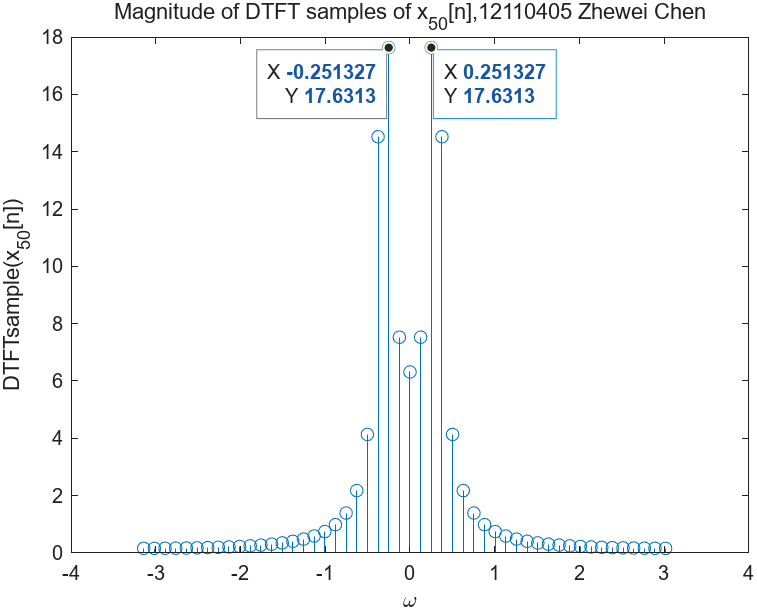
\includegraphics[width=0.4\textwidth]{523.png} % 将"your_image.png"替换为您的PNG图片文件名
\caption{Plot of DTFTsamples when N = 50}
   \label{fig:3}
 \end{figure}
\begin{figure}[htbp]
   \centering  
   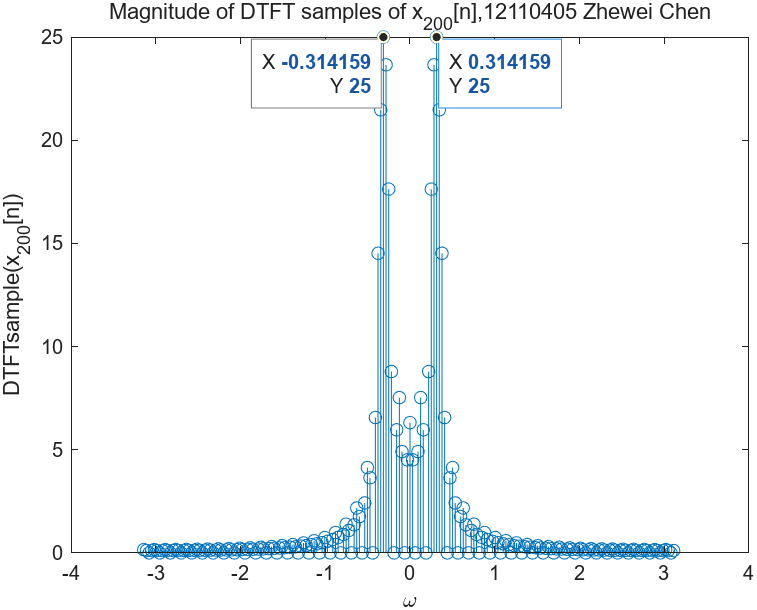
\includegraphics[width=0.4\textwidth]{524.png} % 将"your_image.png"替换为您的PNG图片文件名
\caption{Plot of DTFTsamples when N = 200(with zero padding)}
   \label{fig:4}
 \end{figure}

 $~$

 \textcolor[rgb]{0,0.6,1}{Analysis:}

 \textcolor[rgb]{0,0.6,1}{1 -} Plot of case $\mathbf{N=200}$ (with zero padding) looks more similar to the true DTFT plot than case $N=50$.

 \textcolor[rgb]{0,0.6,1}{2 -} The reasons why two plots look so different:

Firstly, we need to derive how the true DTFT plot looks like.According to the last DFT lab, we can know that $x[n]$ can be a truncated function of $y[n]=\sin (0.1\pi n), -\infty<n<\infty$ 
,with window function $\omega[n]=1, 0 \leq n \leq 49$.

$~$

\(\displaystyle X(e^{j\omega})=Y(e^{j\omega})*W(e^{j\omega})\)\\
\(\displaystyle ~~~~~~~~~~~~=(\pi\delta(\omega-0.1\pi)+\pi\delta(\omega+0.1\pi))W(e^{j\omega})\)\\
\(\displaystyle  ~~~~~~~~~~~~=\pi W(e^{j(\omega-0.1\pi)})+\pi W(e^{j(\omega+0.1\pi)})\)

Again, according to the last lab,

$~$

\(\displaystyle W\left(e^{j \omega}\right)=e^{-j \omega(N-1) / 2} \frac{\sin (\omega N / 2)}{\sin (\omega / 2)}\)

So we can derive that $X(e^{j\omega})$ is composed of two shifted sinc functions, centered at $\omega = 0.1\pi$ and $\omega = -0.1\pi$ respectively.

Both Fig. 3 and Fig. 4 are the frequency samples of $X(e^{j\omega})$. 
However, Fig.4 show more details(for example, the two peak of DTFTsamples is closer to the true DTFT) of $X(e^{j\omega})$ than Fig.3, because the $\mathbf{frequency~resolution}$ of Fig.4 is higher than Fig.3.

$~$

\textcolor[rgb]{0,0.6,1}{3 -} The reasons why case N =200 (with zero padding) can provide higher $\mathbf{frequency~resolution}$:


Recall the mathematical definition of DFT and DTFT, we can know that DFT is frequency sampling of DTFT at $\omega=2\pi k/N, k=0,1,...,N-1$, which also means DFT has a frequency resolution of $\omega=2\pi k/N$.

When we increase the length of $x[n]$ with zero padding, it will $\mathbf{not}$ change the value of $X_N[k]$.Because the data we add into $x_N[k]$ is zero.
However the $\omega=2\pi k/N$ will be more dense, which means the frequency resolution will be $\mathbf{higher}$.

So the case N =200 (with zero padding) can provide higher frequency resolution and is similar to the true DTFT plot.

\subsection{The Fast Furier Transform}
\subsubsection{Implementation of Divide-and-Conquer DFT}
$~$

This section we will implement the divide-and-conquer DFT algorithm in Matlab.
 According to the lab manual, the divide-and-conquer DFT algorithm is as follows:

\[
   \scalebox{0.9}{
$\begin{rcases}
 X[k] = X_0[k] + W_N^k X_1[k] \\
X[k + N/2] = X_0[k] - W_N^k X_1[k]
\end{rcases}
\text{for } k = 0,..\frac{N}{2} - 1$
   }
\]
where the complex constants defined by \(W_N^k = e^{-j2\pi k/N}\)  are called twiddle factors.
We can use digram to illustrate the divide-and-conquer DFT algorithm as Fig. 5.
\begin{figure}[htbp]
   \centering
   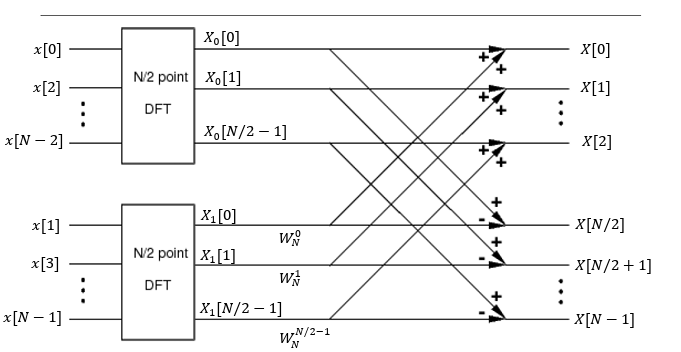
\includegraphics[width=0.42\textwidth]{531.png} % 将"your_image.png"替换为您的PNG图片文件名
\caption{DIgram of divide and conquer DFT of N-point, computed using the two N/2-point DFT's $X_0^{N/2}[k]~$  and$ X_1^{N/2}[k]$}
   \label{fig:0}
 \end{figure}
\begin{lstlisting}[title={dcDFT.m},style=Matlab-editor]
   function X = dcDFT(x)
   N=length(x);
   x0=x(1:2:N);% even part
   x1=x(2:2:N);% odd part
   X0=DFTsum(x0);
   X1=DFTsum(x1);
   k=0:1:N/2-1;
   twiddle_factor=exp(-1i*2*pi*k/N);
   X1=twiddle_factor.*X1;
   X=[X0+X1 X0-X1];
   end
\end{lstlisting}
\begin{lstlisting}[title={DFTsum.m},style=Matlab-editor]
   function X = DFTsum(x)
   N = length(x);
   X = zeros(1,N);
   for k=1:N
      for n=1:N
         X(k)= X(k)+x(n)*exp(-1i*2*pi*(k-1)*(n-1)/N);
      end
   end
   end
\end{lstlisting}

$~$

Then we test the functions by input signal 

$~$

$x_1[n]=\delta[n], \text{for}\ N=10$

$x_2[n]=1, \text{for}\ N=10$

$x_3[n]=e^{j2\pi n/N}, \text{for}\ N=10$

$~$

and compare the results computed by $\mathbf{DFTsum.m}$ and $\mathbf{dcDFT.m}$
(The $\mathbf{DFTsum.m}$ is a direct implementation of DFT and it is from the last lab.)
$~$
\begin{figure}[htbp]
   \centering
   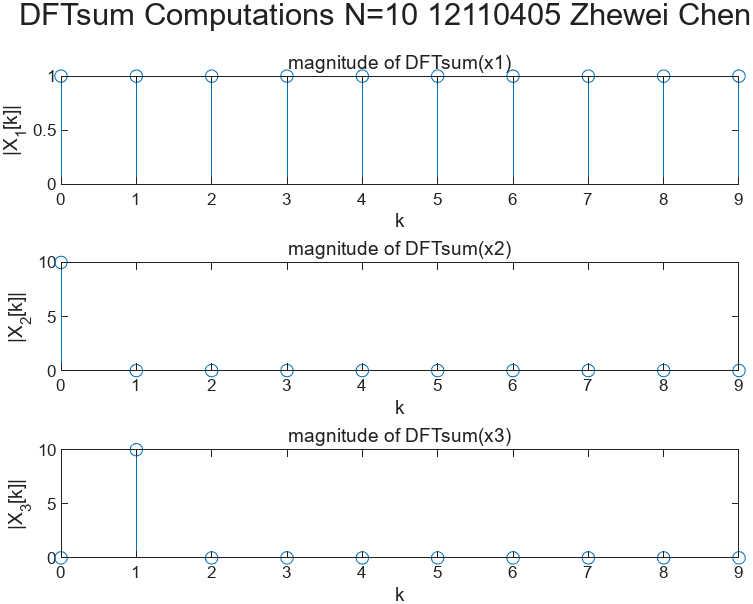
\includegraphics[width=0.5\textwidth]{5311.png} % 将"your_image.png"替换为您的PNG图片文件名
\caption{Plot of the calculation results of $\mathbf{DFTsum.m}$ for $x_1[n]$,$x_2[n]$,$x_3[n]$ with $N$=10}
   \label{fig:5}
 \end{figure}

\begin{figure}[htbp]
   \centering
   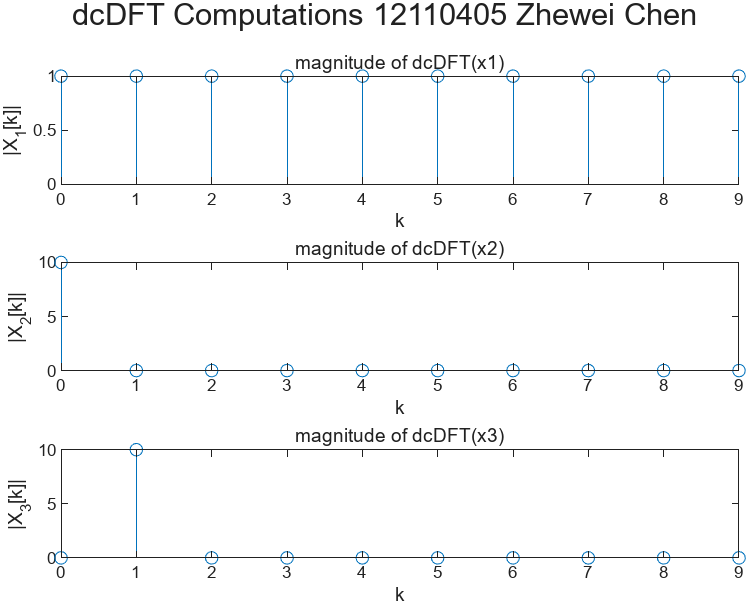
\includegraphics[width=0.5\textwidth]{5312.png} % 将"your_image.png"替换为您的PNG图片文件名
\caption{Plot of the calculation results of $\mathbf{dcDFT.m}$ for $x_1[n]$,$x_2[n]$,$x_3[n]$ with $N$=10}
   \label{fig:6}
\end{figure}

$~$

\textcolor[rgb]{0,0.6,1}{Analysis:}

$~$

\textcolor[rgb]{0,0.6,1}{1 -}The results computed by $\mathbf{DFTsum.m}$ and $\mathbf{dcDFT.m}$ are the same. In function $\mathbf{dcDFT.m}$,
 we divide the input signal into even and odd parts, and then compute the DFT of each part. Finally, we combine the results of the two parts to get the result.
 
\textcolor[rgb]{0,0.6,1}{2 -}
The number of multiplies that are required in this approach to computing an $N$
point DFT is $\mathbf{(N+N^2)/2}$. (Consider a multiply to be one multiplication of real or complex numbers.) 

So the total number of multiplications is $(N+N^2)/2$.
For two parts $N/2$-point DFT, we need two of $(N/2)^2$ multiplications.
To simplify, we also consider constant twiddle factor (for example,1,-1) as one multiplication. So we need $N/2$ multiplications for twiddle factor. Because the in $\mathbf{dcDFT.m}$ we only need to compute the twiddle factor in the range of $k=0,1,...,N/2-1$.
So the total number is $(N/2)^2 \times2+N/2=(N+N^2)/2$.

$~$

\subsubsection{Recursive Divide and Conquer }
$~$

In this section we will implement the divide-and-conquer algorithm recursively, that means recursively divide the DFT computations until the length of the sequence is 2 and then combine the results.
Using this algorithm, we write MATLAB functions $\mathbf{FFT2.m}$, $\mathbf{FFT4.m}$, $\mathbf{FFT8.m}$ to compute the FFT of lengths 2, 4, 8 respectively.

$~$

$~$

\begin{lstlisting}[title={FFT2.m},style=Matlab-editor]
   function X = FFT2(x)
   X(1)=x(1)+x(2);
   X(2)=x(1)-x(2);
   end   
\end{lstlisting}

\begin{lstlisting}[title={FFT4.m},style=Matlab-editor]
   function X = FFT4(x)
   N=4;%N=length(x);
   x_even=x(1:2:N);  X_even=FFT2(x_even);
   x_odd=x(2:2:N);   X_odd=FFT2(x_odd);
   k=0:N/2-1;
   twiddle_factor=exp(-1i*2*pi*k/N);
   X_odd=twiddle_factor.*X_odd;
   X=[X_even+X_odd   X_even-X_odd];
   end
\end{lstlisting}

\begin{lstlisting}[title={FFT8.m},style=Matlab-editor]
   function X = FFT8(x)
   N=8;%N=length(x);
   x_even=x(1:2:N);  X_even=FFT4(x_even);
   x_odd=x(2:2:N);   X_odd=FFT4(x_odd);
   k=0:N/2-1;
   twiddle_factor=exp(-1i*2*pi*k/N);
   X_odd=twiddle_factor.*X_odd;
   X=[X_even+X_odd   X_even-X_odd];
   end
\end{lstlisting}

\begin{lstlisting}[title={fftstage.m},style=Matlab-editor]
   function X = fftstage(x)
   N=length(x);
   x_even=x(1:2:N);
   X_even=fftstage(x_even);
   x_odd=x(2:2:N); X_odd=fftstage(x_odd);
   k=0:N/2-1;
   twiddle_factor=exp(-1i*2*pi*k/N);
   X_odd=twiddle_factor.*X_odd;
   X=[X_even+X_odd   X_even-X_odd];
   end
\end{lstlisting}

Then we test the functions by input signal :

$~$

$x_1[n]=\delta[n], \text{for}\ N=8$

$x_2[n]=1, \text{for}\ N=8$

$x_3[n]=e^{j2\pi n/N}, \text{for}\ N=8$

and compare the results computed by $\mathbf{DFTsum.m}$ and $\mathbf{FFT8.m}$ 


\begin{figure}[htbp]
   \centering
   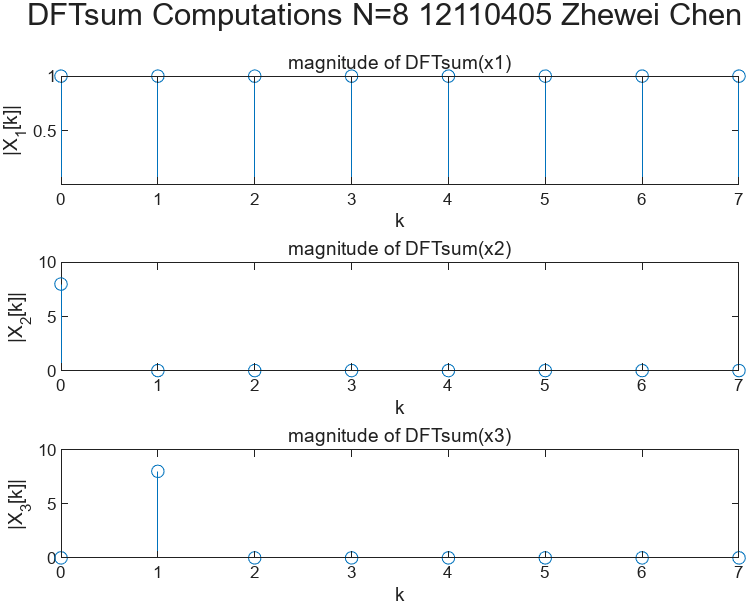
\includegraphics[width=0.35\textwidth]{5321.png} % 将"your_image.png"替换为您的PNG图片文件名
\caption{Plot of the calculation results of $\mathbf{DFTsum.m}$ for $x_1[n]$,$x_2[n]$,$x_3[n]$ with $N$=8}
   \label{fig:7}
\end{figure}

\begin{figure}[htbp]
   \centering
   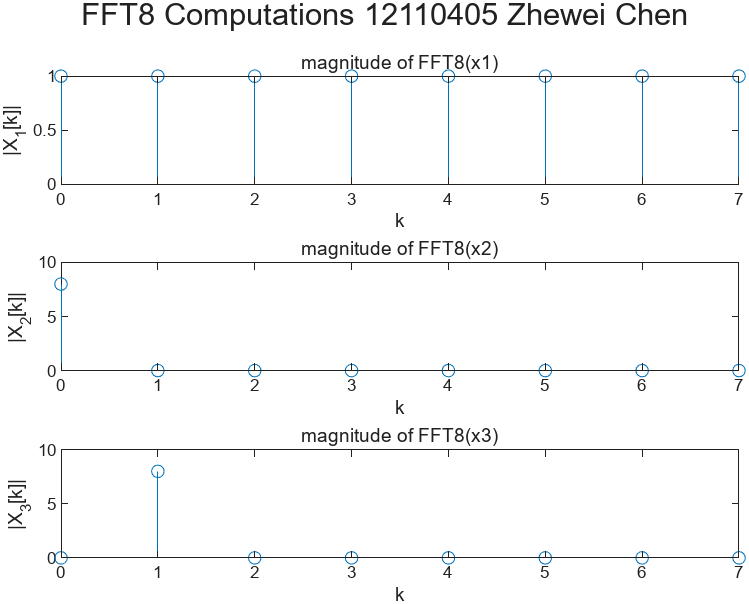
\includegraphics[width=0.44\textwidth]{5322.png} % 将"your_image.png"替换为您的PNG图片文件名
\caption{Plot of the calculation results of $\mathbf{FFT8.m}$ for $x_1[n]$,$x_2[n]$,$x_3[n]$ with $N$=8}
   \label{fig:8}
 \end{figure}


 \begin{figure}[htbp]
   \centering
   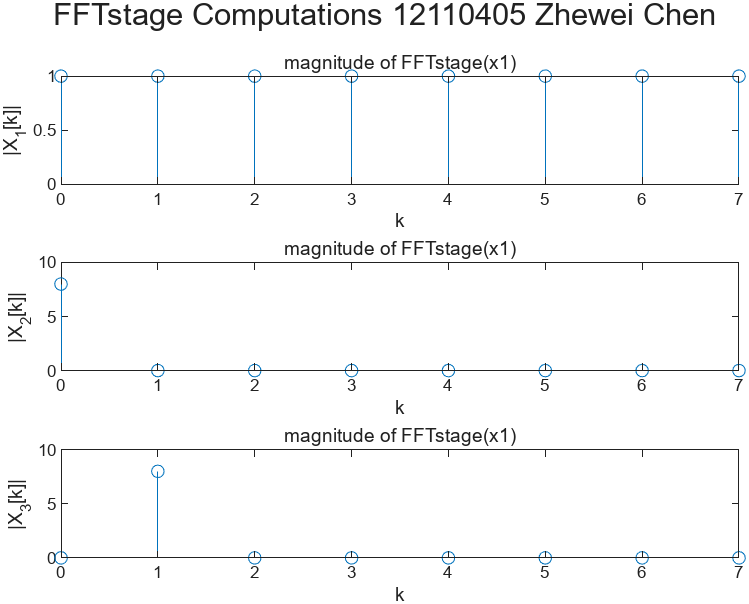
\includegraphics[width=0.4\textwidth]{5323.png} % 将"your_image.png"替换为您的PNG图片文件名
\caption{Plot of the calculation results of $\mathbf{fftstage.m}$ for $x_1[n]$,$x_2[n]$,$x_3[n]$ with $N$=8}
   \label{fig:9}
 \end{figure}

 \textcolor[rgb]{0,0.6,1}{Analysis:}

   $~$

\textcolor[rgb]{0,0.6,1}{1 -}The results computed by $\mathbf{DFTsum.m}$, $\mathbf{FFT8.m}$ and $\mathbf{fftstage}$ are the same. 
In function $\mathbf{FFT8.m}$, we compute the half DFTs with $\mathbf{FFT4.m}$, and in function $\mathbf{FFT4.m}$, we compute the half DFTs with $\mathbf{FFT2.m}$.
In function $\mathbf{fftstage.m}$, we compute the half DFTs with $\mathbf{fftstage.m}$ recursively. 

$~$

$~$

$~$

\textcolor[rgb]{0,0.6,1}{2 -}

\begin{figure}[H]
   \centering
   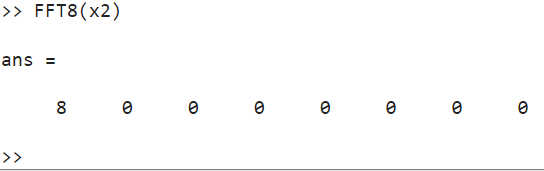
\includegraphics[width=0.4\textwidth]{5324.png} % 将"your_image.png"替换为您的PNG图片文件名
\caption{Result of $\mathbf{FFT8.m}$ with input signal $x_2[n]$,for $N$=8}
   \label{fig:10}
 \end{figure}

 \textcolor[rgb]{0,0.6,1}{3 -}The total number of multiplies by twiddle factors required for 8-point FFT(A multiply is a multiplication by a real or complex number.) :
 $8/2\times\log_2 8=$$\mathbf{12}$.(Including considering $W_N^0=1$ and $W_2^{1}=-1$ as one multiplication respectively)

 \textcolor[rgb]{0,0.6,1}{4 -}
Including considering constant twiddle factors like $W_N^0=1$ as one multiplication:

A formula for the number of multiplies required for an $N = 2^p$ point FFT : $\mathbf{(Nlog_{2}N)/2}$ or $\mathbf{p2^{p-1}}$

As we derive the number of multiplies required $\mathbf{dcDFT.m}$ with length $N$ input signal.
We do the $\displaystyle log_{2} N$ times divisions, each division increase $N/2$ multiplies. So the total number of multiplies is $(Nlog_{2}N)/2$ or $p2^{p-1}$.


Consider a $p=10$ DFT.Compared to number of multiplies required for direct implementation needs $N^2=2^{2p}$=1048576 multiplications,  FFT just needs $10\times 2^9=5120$ multiplications 
\section{Expasion Content}
If a signal is not in the form of $N = 2^p$, we can use zero padding to expand the signal to the form of $N = 2^p$.
\begin{lstlisting}[title={zeropadding.m},style=Matlab-editor]
   function [y] = zeropadding(x)
   N=length(x);
   nextPowerOf2 = nextpow2(N);  
   N1 = 2^nextPowerOf2;
   y = [x, zeros(1, N1 - N)];
   end
\end{lstlisting}
\begin{figure}[htbp]
   \centering
   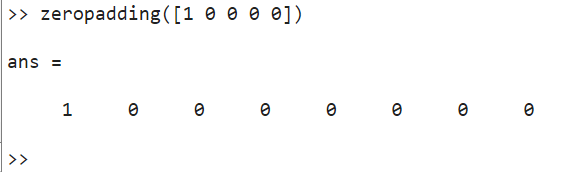
\includegraphics[width=0.5\textwidth]{54.png} % 将"your_image.png"替换为您的PNG图片文件名
\caption{Test for $\mathbf{zeropadding.m}$}
   \label{fig:12}
 \end{figure}

Then we can use our $\mathbf{fftstage.m}$ to compute the FFT of lengths $N$, where $N=1,2,3\dots$.

\textcolor[rgb]{0,0.6,1}{Analysis:}

Though zero padding means more computation, it has fewer effect on complexity than the decrease of the number of multiplications that FFT provided. At the same time, zero padding can increase the frequency resolution to make the DFT image more closely resemble the actual DTFT image. So it is worthy using zero padding to expand the signal to implement FFT.
\section{Conclusion}
During this lab, we study that we can use function to shift DFT frequency domain and change the scale of the horizontal axis from $k$ to $\omega$ of DFT plots. By zero-padding, we can increase the frequency resolution to make the DFT image more closely resemble the actual DTFT image.
We researched how to using the method of divide and conquer to recursively implement the Fast Fourier Transform (FFT), which could lead to a extremely decrease the number of multiplications.
Also we learned how to use zero padding to expand the signal to the form of $N = 2^p$ to compute the FFT of lengths $N$, where $N=1,2,3\dots$.
In this lab, we tried a method to $\mathbf{combine}$ mathematical derivation and MATLAB programming to study ot plot the results of DFT and FFT, which helps us to understand the computation of DFT and FFT $\mathbf{theriotically}$ and $\mathbf{practically}$.
\end{document}
